\subsection{Exact points: how the single constant $\kappa$ is found}
The loss counts, for every soil, how many decades the predicted reach lies outside the interval observed in the simulations (zero when inside), squared and summed. The constant is the value of $\kappa$ at the bottom of this curve.
\begin{center}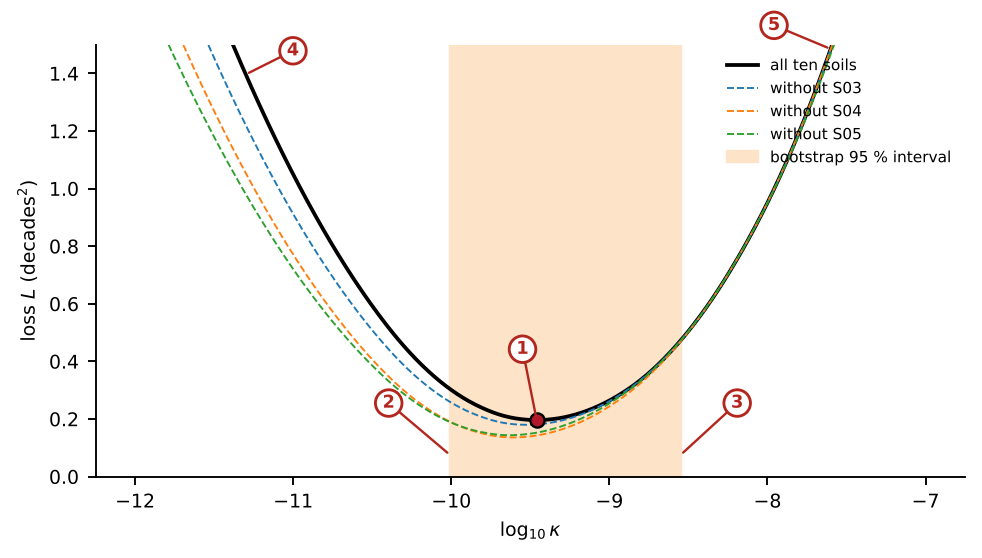
\includegraphics[width=0.92\textwidth]{../figures/paper4/ex_kappa.png}\end{center}
\textbf{What the numbered labels point to, with the exact values.}
\begin{enumerate}[nosep,label=\protect\circled{\arabic*}]
\item The minimum: $\log_{10}\kappa=-9.46$, $\kappa=3.47\times10^{-10}$, loss $L=0.196$\,decades$^2$. At this value 5 soils lie outside their interval: S01 by 0.11 decade, S02 by 0.27 decade, S03 by 0.12 decade, S04 by 0.23 decade, S05 by 0.21 decade; the other 5 lie inside.
\item Left edge of the bootstrap interval, $\kappa=9.8e-11$: resampling the ten soils with replacement 1\,000 times and refitting.
\item Right edge, $\kappa=2.8e-09$. The interval spans 1.5 decades, but the reach changes only by a factor 1.45 to 2.45 per decade of $\kappa$.
\item Too small a $\kappa$ puts every predicted reach too far into the dry range: the soils with a finite interval (sand, loamy sand, sandy loam) are missed and the loss rises.
\item Too large a $\kappa$ predicts reaches that are too short: soils whose triggers fire up to $10^4$\,cm are missed.
\end{enumerate}
\textbf{How the exact points are obtained from the data.} The observed intervals are the columns \texttt{reach\_observed\_low\_cm} and \texttt{reach\_observed\_high\_cm} of Table~A1, from experiment E2 (next graph). The predicted reach for each trial $\kappa$ is \cref{eq:s-hc}. The minimum was found with the Nelder--Mead method in \nolinkurl{p4_reach.py} (function \texttt{fitm}); the bootstrap and the curves without one soil are in \nolinkurl{p4_numbers.json} under \texttt{constants}. The flat bottom of the curve is why $\kappa$ is uncertain by a decade while the reaches are not: every reach depends on $\kappa$ only through the power $1/[2n+\ell(n-1)]$.
